\documentclass[a4paper, 12pt]{article}%тип документа

%отступы
\usepackage[left=2cm,right=2cm,top=2cm,bottom=3cm,bindingoffset=0cm]{geometry}

%Русский язык
\usepackage[T2A]{fontenc} %кодировка
\usepackage[utf8]{inputenc} %кодировка исходного кода
\usepackage[english,russian]{babel} %локализация и переносы

%Вставка картинок
\usepackage{wrapfig}
\usepackage{graphicx}
\graphicspath{{pictures/}}
\DeclareGraphicsExtensions{.pdf,.png,.jpg}

%Графики
\usepackage{multirow}
\usepackage{pgfplots}
\pgfplotsset{compat=1.9}

%Математика
\usepackage{amsmath, amsfonts, amssymb, amsthm, mathtools}

%Заголовок
\author{Сифат Мд Абдуллах Ал Хасиб  \\
Факультет физической и квантовой электроники \\
Группа Б04-105}
\title{\textbf{ВОПРОС ПО ВЫБОРУ \\ 
Экспериментальная модель для измерения теплопроводности Методом Горячей проволоки}}
\begin{document}
\maketitle
\begin{abstract}
Тепловой поток $J_r$ имеет отношение к данному теплу в системе. Из этого соотношения я вывел формулу, по которой мы можем найти теплопроводность. В этой статье я объяснил небольшой эксперимент, касающийся теории, а позже я описал важное применение этого метода в Вакуумметр Пирани, который обычно используется в вакуумных системах для измерения давления.
\end{abstract}
\section{Общая теория}
Мы можем определить тепло как тепловую энергию в пути. Он количественно определяет передачу энергии в ответ на температурный градиент. Количество тепла, которое проходит вдоль температурного градиента, зависит от теплопроводности материала, которую мы сейчас определим. Теплопроводность можно рассматривать в одном измерении, используя диаграмму, показанную на рис.1. Тепло течет от горячего к холодному и, таким образом, течет против температурного градиента. Поток тепла может быть описан вектором теплового потока J, направление которого лежит вдоль направления потока тепла и величина которого равна тепловой энергии, протекающей в единицу времени на единицу площади (измеряется в $Js ^{-1}m^{-2} = Wm^{-2}$). Тепловой поток $J_z$ в направлении z задается формулой
\begin{center}
$J_z = -\kappa(\frac{\partial T}{\partial z})$
\end{center}
где отрицательный знак это потому что тепло течет вниз по склону. Постоянная $\kappa$ называется теплопроводностью газа. В общем, в трех измерениях мы можем записать, что тепловой поток $ J $ связан с температурой, используя
\begin{center}
$J = -\kappa \nabla T$
\end{center}

\begin{figure}[h]
\begin{center}
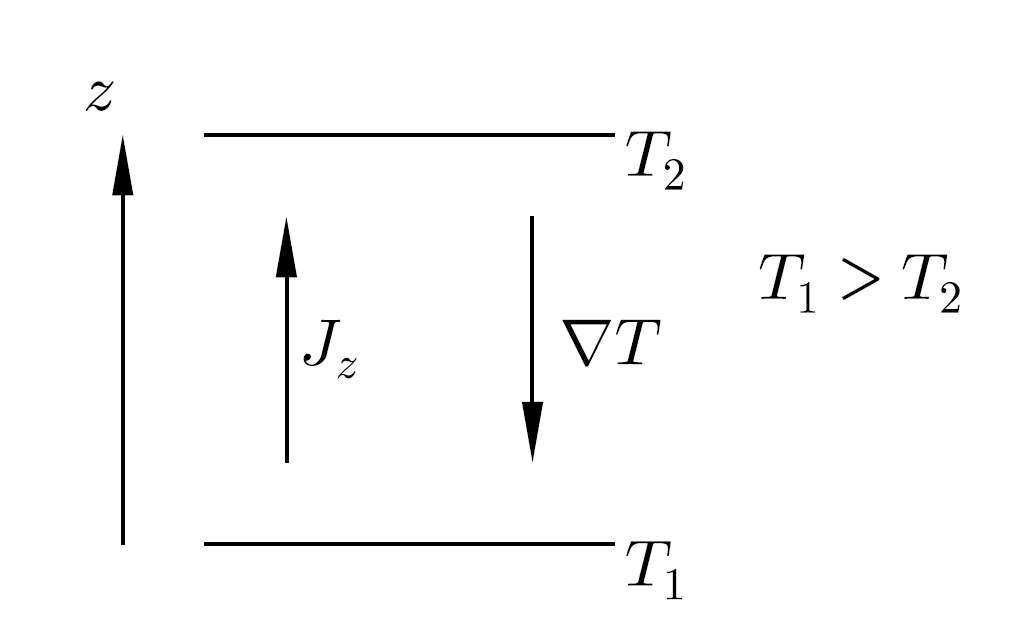
\includegraphics[width = 0.8\textwidth]{Bigar 1.png}
\caption{Тепло течет в направлении, противоположном градиенту температуры.}
\end{center}
\end{figure}
\newpage
\section{Измерение теплопроводности} 
Теплопроводность $\ kappa$ можно измерить с помощью метода горячей проволоки. Газ заполняет пространство между двумя коаксиальными цилиндрами (внутренний радиус цилиндра a, внешний радиус цилиндра b), как показано на фиг.2. Внешний цилиндр соединен с ванной постоянной температуры с температурой $T_b$, в то время как во внутреннем цилиндре (горячая проволока) выделяется тепло со скоростью Q на единицу длины цилиндра (измеряется в единицах $ Wm ^ {-1}$. Температура внутреннего цилиндра повышается до $T_a$. Скорость $Q$ может быть связана с радиальным тепловым потоком $J_r$ с помощью
\begin{center}
$Q = 2 \pi r J_r$
\end{center}
а сам $J_r$ задается через $-\kappa \frac{\partial T}{\partial r}$, как в первом уравнении. Следовательно,
\begin{center}
$Q = {-2} \pi r \kappa \frac{\partial T}{\partial r} $
\end{center}
Перегруппировка и интегрирование дают
\begin{center}

$Q \int_{a}^{b} \frac{dr}{r} = -2\pi\kappa\int_{T_a}^{T_b}dT $
\end{center}
and hence
\begin{center}
$\kappa = \frac{Q}{2\pi}\frac{ln(b/a)}{T_a - T_b} $
\end{center}
Поскольку $Q$ известен (это мощность, подаваемая для нагрева внутреннего цилиндра) и $T_a$ и $T_b$ могут быть измерены, можно вывести значение $\kappa$.
\begin{figure}[h]
\begin{center}
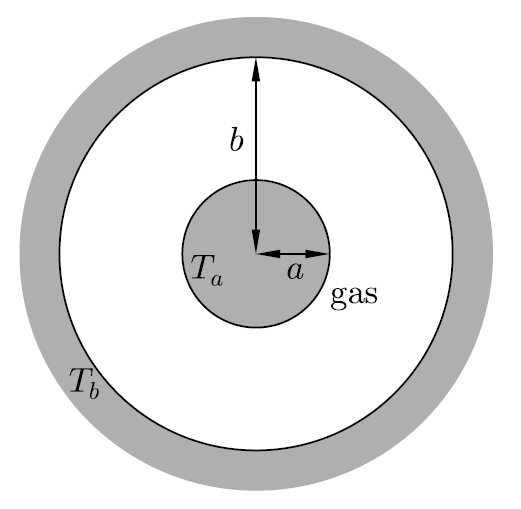
\includegraphics[width = 0.8\textwidth]{B3.png}
\caption{Метод измерения теплопроводности с помощью горячей проволоки}
\end{center}
\end{figure}
\newpage
\section{Вакуумметр Пирани} Вакуумметр Пирани - это надежный датчик теплопроводности, используемый для измерения давления в вакуумных системах. Он был изобретен в 1906 году Марчелло Пирани. Важным применением этого метода является Вакуумметр Пирани, который обычно используется в вакуумных системах для измерения давления. Провод датчика нагревается электрически, и давление газа определяется путем измерения тока, необходимого для поддержания постоянной температуры провода. (Сопротивление провода зависит от температуры, поэтому температура оценивается путем измерения сопротивления провода.) Таким образом, Вакуумметр Пирани основан на том факте, что при низком давлении теплопроводность является функцией давления (поскольку условие $\lambda \ll L$, где $L$ - линейный размер в манометре, не выполняется). На самом деле, типичный Вакуумметр Пирани не будет работать для определения давления намного выше 1 мбар, потому что при превышении этих давлений теплопроводность газов больше не изменяется с давлением. Теплопроводность каждого газа различна, поэтому датчик должен быть откалиброван для конкретного измеряемого газа. На рисунке ниже я просто привожу фотографию структурной схемы Вакуумметр Пирани без подробного обсуждения.
\begin{figure}[h]
\begin{center}
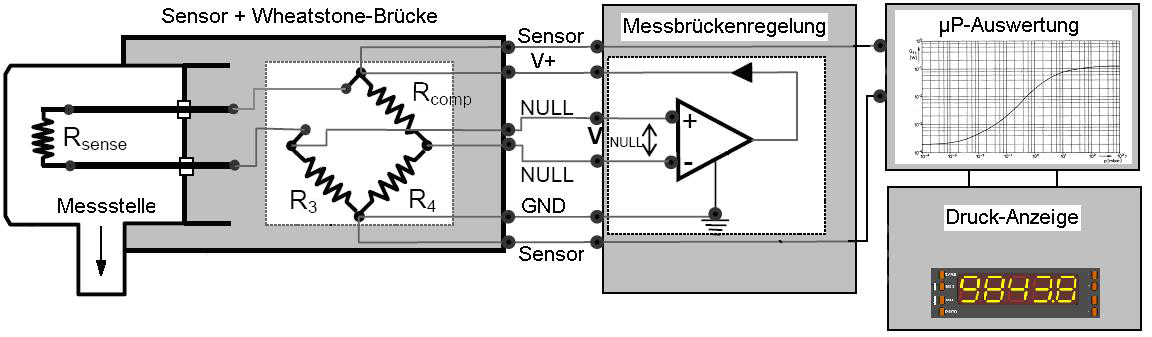
\includegraphics[width = 0.8\textwidth]{B2.png}
\caption{Структурная схема Вакуумметр Пирани}
\end{center}
\end{figure}
\newpage
\section{Вывод} 
Мы можем найти теплопроводность, используя другой метод. Среди них метод горячей проволоки имеет очень практическое применение. Я только что показал основную схему эксперимента на рисунке 2. Когда мы будем проводить эксперимент, мы должны сначала измерить радиус двух цилиндров и температуру внешнего цилиндра и решить, сколько тепла мы отдадим системе. Затем мы можем получить табличное значение теплопроводности, а затем сравнить то, что мы получаем в результате нашего эксперимента. Здесь мы должны рассмотреть металл, из которого изготовлены цилиндры. 


\end{document}